
\pgfplotsset{
%        compat=newest,  % <-- does not work; don't know why
        compat=1.13,     % <-- works as expected
    }
  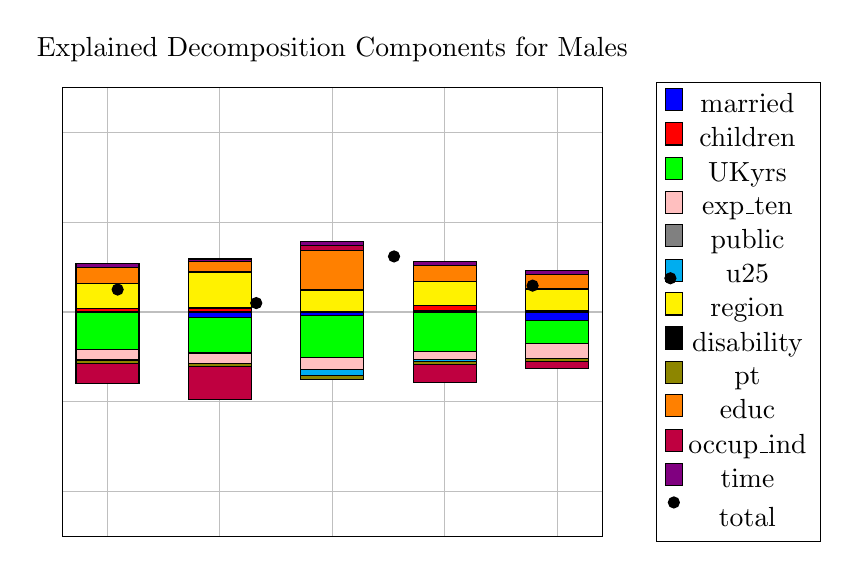
\begin{tikzpicture}
  %\node [align=center, font=\small, rotate=45,text width=2.15cm, inner sep=0.25cm] at (1, 1) {\textsc{year 1}};
  \begin{axis}[
    title={Explained Decomposition Components for Males},
    ybar stacked,
    ymax=0.5,
    ymin=-0.5,
    ymajorgrids = true,
    xmajorgrids = true,
    bar width=8mm,
    %xtick={1,2,3,4,5},
    %xticklabels={White, Black, Chinese, Asian, Mixed}
    symbolic x coords={Non-white, Black, Chinese, Asian, Mixed},
    xtick=data,
    nodes near coords align={anchor=north},%Move values in bar
    every node near coord/.style={},
    legend style={at={(1.1,0.5)},anchor=west}
  ]
%married
\addplot [fill=blue] coordinates {({Non-white},-0.0016696)({Black},-0.0114677)({Chinese},-0.0073378)({Asian},0.0043633)({Mixed},-0.0193238)};
%children
\addplot [fill=red] coordinates {({Non-white},0.0076544)({Black},0.0072453)({Chinese},-0.0001029)({Asian},0.0103292)({Mixed},0.000237)};
%UKyrs
\addplot [fill=green] coordinates {({Non-white},-0.0827489)({Black},-0.0798941)({Chinese},-0.094151)({Asian},-0.0876264)({Mixed},-0.049982)};
%exp_ten
\addplot [fill=pink] coordinates {({Non-white},-0.0205585)({Black},-0.0236869)({Chinese},-0.0271182)({Asian},-0.0175927)({Mixed},-0.0337114)};
%public
\addplot [fill=gray] coordinates {({Non-white},-0.0000177)({Black},0.000134)({Chinese},0.0000439)({Asian},-0.0001873)({Mixed},0.0000368)};
%u25
\addplot [fill=cyan] coordinates {({Non-white},-0.0029587)({Black},0.0015461)({Chinese},-0.0133931)({Asian},-0.0041728)({Mixed},0.0019511)};
%region
\addplot [fill=yellow] coordinates {({Non-white},0.0556098)({Black},0.0789507)({Chinese},0.0479198)({Asian},0.0525374)({Mixed},0.048946)};
%disability
\addplot [fill=black] coordinates {({Non-white},0.0010224)({Black},0.001942)({Chinese},0.0025078)({Asian},0.0007863)({Mixed},0.0003095)};
%pt
\addplot [fill=olive] coordinates {({Non-white},-0.0072398)({Black},-0.0065685)({Chinese},-0.0083853)({Asian},-0.0077012)({Mixed},-0.0065703)};
%educ
\addplot [fill=orange] coordinates {({Non-white},0.0353103)({Black},0.0224164)({Chinese},0.0859756)({Asian},0.0362466)({Mixed},0.0331086)};
%occup_ind
\addplot [fill=purple] coordinates {({Non-white},-0.044695)({Black},-0.0736681)({Chinese},0.0121925)({Asian},-0.0403711)({Mixed},-0.0159515)};
%time
\addplot [fill=violet] coordinates {({Non-white},0.0077757)({Black},0.0059754)({Chinese},0.0094211)({Asian},0.0079897)({Mixed},0.0088938)};

\addplot [only marks,mark=*,mark size=2pt,black,
         nodes near coords = \rotatebox{90}{{\pgfmathprintnumber[fixed zerofill,
                                    precision=2]{\pgfplotspointmeta}}},
        nodes near coords align={vertical},
        point meta=y,
        every node near coord/.append style={font=\small, yshift=0.25mm},] coordinates {({Mixed},-1)};
%\begin{comment}
%\end{comment}
%\filldraw[black] (0,0) circle (2pt) node[anchor=west] {Intersection point};
  \legend{married, children, UKyrs, exp\_ten, public, u25, region, disability, pt, educ, occup\_ind, time, total}
  \end{axis}
  
  \begin{axis}[
    nodes near coords align={anchor=north},%Move values in bar
    every node near coord/.style={},
    xtick=data,
    ymax=0.3,
    ymin=-0.3,
    xmax=0,
    xmin=5,
]
\pgfplotsset{ticks=none}
\addplot[only marks,mark=*,mark size=3pt,black,
         nodes near coords = \rotatebox{90}{{\pgfmathprintnumber[fixed zerofill,
                                    precision=2]{\pgfplotspointmeta}}},
        nodes near coords align={vertical},
        point meta=y,
        every node near coord/.append style={font=\small, yshift=0.25mm},
        ]  coordinates {
    (1,0.1) (2,-0.1) (3,1)
};
\end{axis}
\filldraw[black] (0.7,3.1323929) circle (2pt) node[anchor=west] {};
\filldraw[black] (2.46,2.9604722) circle (2pt) node[anchor=west] {};
\filldraw[black] (4.21,3.5530061) circle (2pt) node[anchor=west] {};
\filldraw[black] (5.97,3.1822077) circle (2pt) node[anchor=west] {};
\filldraw[black] (7.72,3.2756059) circle (2pt) node[anchor=west] {};
  \end{tikzpicture}
